\section{Đặc tả thanh ghi}\label{sec:2}

Firmware dựng chuỗi descriptor trong DRAM, ghi \sig{DESC_PTR}, thực hiện \sig{fence rw,rw}, ghi
START (\sig{CTRL[2]}), rồi đọc \sig{STATUS} cho tới khi DONE hoặc ERROR bằng 1. Tham số của từng
phép GEMM nằm trong descriptor (mục~\ref{sec:5.2}), không nằm trong thanh ghi MMIO. Offset
0x08 … 0x24 dự trữ.

\subsection{Tổng hợp thanh ghi}\label{sec:2.1}
Địa chỉ tuyệt đối = \sig{MMIO_BASE} + offset; vùng MMIO 4 KiB tại 0x6000\_0000, tức
0x6000\_0000 … 0x6000\_0FFF. Thanh ghi căn word; phần cứng chỉ giải mã bit địa chỉ [11:2].
RW: đọc/ghi theo byte; RO: chỉ đọc, ghi bị bỏ qua; W: ghi lệnh, đọc luôn bằng 0. Không có bit RW1C.
Các offset không liệt kê đọc 0, ghi bị bỏ qua, phản hồi luôn OKAY.
\begin{spectable}{|L{0.15}|L{0.3}|L{0.55}|}{Tổng hợp thanh ghi}{tab:2-1}{\textbf{Offset} & \textbf{Tên viết tắt} & \textbf{Tên thanh ghi}}
0x00 & CTRL\_REG & Thanh ghi điều khiển \\\hline

0x04 & STATUS\_REG & Thanh ghi trạng thái \\\hline

0x08 … 0x24 & — & Reserved \\\hline

0x28 & HW\_CONFIG & Cấu hình phần cứng \\\hline

0x2C & PERF\_TOTAL & Tổng số chu kỳ BUSY của tác vụ \\\hline

0x30 & PERF\_LOAD & Số chu kỳ LOAD, không tính FETCH \\\hline

0x34 & PERF\_COMPUTE & Số chu kỳ COMPUTE \\\hline

0x38 & PERF\_STORE & Số chu kỳ STORE\_C \\\hline

0x3C & — & Reserved \\\hline

0x40 & DESC\_PTR & Con trỏ descriptor đầu \\\hline

0x44 & ERR\_DESC\_ADDR & Địa chỉ descriptor lỗi \\\hline

0x48 & DESC\_DONE\_CNT & Số descriptor hoàn tất \\\hline

Các địa chỉ khác & — & Reserved \\\hline

\end{spectable}

\begin{notebox}[Quyết định baseline D-01]
Offset 0x08 … 0x24 là \textbf{Reserved}. \sig{spec_2} đặt tại đây tám thanh ghi RW của chế độ
single (\sig{MATRIX_DIM}, \sig{BASE_ADDR_IN}, \sig{BASE_ADDR_WEIGHT}, \sig{BASE_ADDR_OUT},
\sig{POST_CTRL}, \sig{BIAS_ADDR}, \sig{QUANT_M0}, \sig{QUANT_SHIFT}); baseline bỏ chế độ đó nên bỏ
luôn tám thanh ghi. Mọi tham số của job lấy từ descriptor. Hệ quả cho firmware: ghi vào
0x08 … 0x24 bị bỏ qua và đọc ra 0, phản hồi vẫn OKAY.
\end{notebox}

\subsection{Thanh ghi điều khiển (CTRL\_REG)}
Địa chỉ offset: 0x00\par
Giá trị reset: 0x0000\_0000\par
\begin{center}
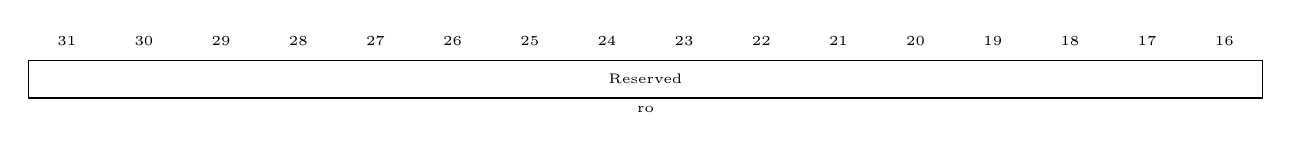
\begin{tikzpicture}[x=0.98cm,y=0.6cm]
\node[font=\tiny] at (0.5,1.2) {31};
\node[font=\tiny] at (1.5,1.2) {30};
\node[font=\tiny] at (2.5,1.2) {29};
\node[font=\tiny] at (3.5,1.2) {28};
\node[font=\tiny] at (4.5,1.2) {27};
\node[font=\tiny] at (5.5,1.2) {26};
\node[font=\tiny] at (6.5,1.2) {25};
\node[font=\tiny] at (7.5,1.2) {24};
\node[font=\tiny] at (8.5,1.2) {23};
\node[font=\tiny] at (9.5,1.2) {22};
\node[font=\tiny] at (10.5,1.2) {21};
\node[font=\tiny] at (11.5,1.2) {20};
\node[font=\tiny] at (12.5,1.2) {19};
\node[font=\tiny] at (13.5,1.2) {18};
\node[font=\tiny] at (14.5,1.2) {17};
\node[font=\tiny] at (15.5,1.2) {16};
\draw (0,0) rectangle (16,0.8);
\node[font=\tiny] at (8.0,0.4) {Reserved};
\node[font=\tiny] at (8.0,-0.25) {ro};
\end{tikzpicture}
\end{center}
\begin{center}
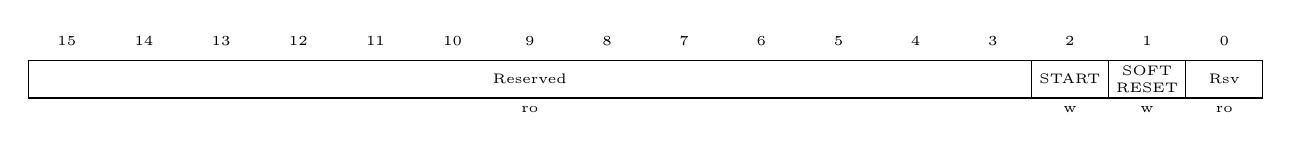
\begin{tikzpicture}[x=0.98cm,y=0.6cm]
\node[font=\tiny] at (0.5,1.2) {15};
\node[font=\tiny] at (1.5,1.2) {14};
\node[font=\tiny] at (2.5,1.2) {13};
\node[font=\tiny] at (3.5,1.2) {12};
\node[font=\tiny] at (4.5,1.2) {11};
\node[font=\tiny] at (5.5,1.2) {10};
\node[font=\tiny] at (6.5,1.2) {9};
\node[font=\tiny] at (7.5,1.2) {8};
\node[font=\tiny] at (8.5,1.2) {7};
\node[font=\tiny] at (9.5,1.2) {6};
\node[font=\tiny] at (10.5,1.2) {5};
\node[font=\tiny] at (11.5,1.2) {4};
\node[font=\tiny] at (12.5,1.2) {3};
\node[font=\tiny] at (13.5,1.2) {2};
\node[font=\tiny] at (14.5,1.2) {1};
\node[font=\tiny] at (15.5,1.2) {0};
\draw (0,0) rectangle (13,0.8);
\node[font=\tiny] at (6.5,0.4) {Reserved};
\node[font=\tiny] at (6.5,-0.25) {ro};
\draw (13,0) rectangle (14,0.8);
\node[font=\tiny] at (13.5,0.4) {START};
\node[font=\tiny] at (13.5,-0.25) {w};
\draw (14,0) rectangle (15,0.8);
\node[font=\tiny,align=center,inner sep=0pt] at (14.5,0.4) {SOFT\\RESET};
\node[font=\tiny] at (14.5,-0.25) {w};
\draw (15,0) rectangle (16,0.8);
\node[font=\tiny] at (15.5,0.4) {Rsv};
\node[font=\tiny] at (15.5,-0.25) {ro};
\end{tikzpicture}
\end{center}
\begin{spectable}{|L{0.09}|L{0.24}|L{0.08}|L{0.15}|L{0.44}|}{Thanh ghi điều khiển}{reg:CTRL_REG}{\textbf{Bit} & \textbf{Tên} & \textbf{Kiểu} & \textbf{Giá trị mặc định} & \textbf{Mô tả}}
31:3 & Reserved & RO & 29'h0 & Đọc 0; ghi bị bỏ qua. \\\hline

2 & START & W & 1'h0 & Ghi 1 bắt đầu chuỗi descriptor tại \sig{DESC_PTR}. Bit tự xóa, đọc luôn ra 0. Chỉ được chấp nhận khi BUSY = 0; khi bận bị bỏ qua, không báo lỗi. \\\hline

1 & SOFT\_RESET & W & 1'h0 & Ghi 1 yêu cầu soft reset (mục~\ref{sec:4.5}); bit tự xóa. Ưu tiên cao hơn START trong cùng một lệnh ghi. \\\hline

0 & Reserved & RO & 1'h0 & Đọc 0; ghi bị bỏ qua. \\\hline

\end{spectable}

\subsection{Thanh ghi trạng thái (STATUS\_REG)}
Địa chỉ offset: 0x04\par
Giá trị reset: 0x0000\_0000\par
\begin{center}
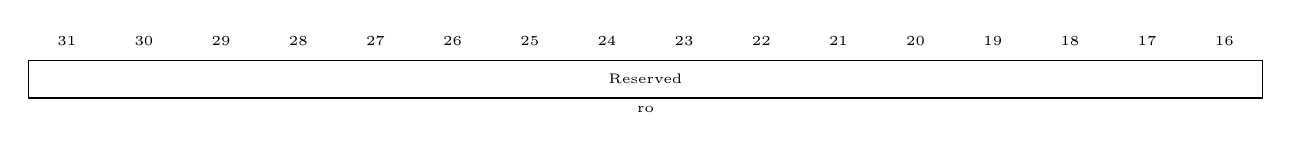
\begin{tikzpicture}[x=0.98cm,y=0.6cm]
\node[font=\tiny] at (0.5,1.2) {31};
\node[font=\tiny] at (1.5,1.2) {30};
\node[font=\tiny] at (2.5,1.2) {29};
\node[font=\tiny] at (3.5,1.2) {28};
\node[font=\tiny] at (4.5,1.2) {27};
\node[font=\tiny] at (5.5,1.2) {26};
\node[font=\tiny] at (6.5,1.2) {25};
\node[font=\tiny] at (7.5,1.2) {24};
\node[font=\tiny] at (8.5,1.2) {23};
\node[font=\tiny] at (9.5,1.2) {22};
\node[font=\tiny] at (10.5,1.2) {21};
\node[font=\tiny] at (11.5,1.2) {20};
\node[font=\tiny] at (12.5,1.2) {19};
\node[font=\tiny] at (13.5,1.2) {18};
\node[font=\tiny] at (14.5,1.2) {17};
\node[font=\tiny] at (15.5,1.2) {16};
\draw (0,0) rectangle (16,0.8);
\node[font=\tiny] at (8.0,0.4) {Reserved};
\node[font=\tiny] at (8.0,-0.25) {ro};
\end{tikzpicture}
\end{center}
\begin{center}
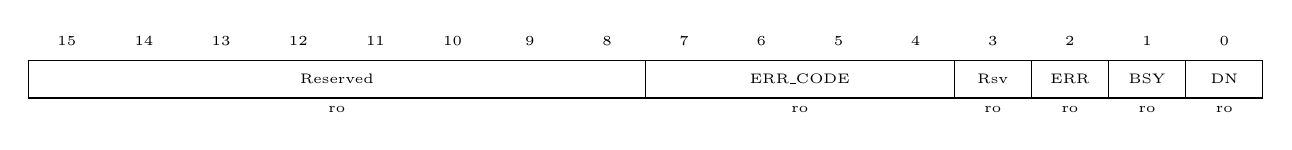
\begin{tikzpicture}[x=0.98cm,y=0.6cm]
\node[font=\tiny] at (0.5,1.2) {15};
\node[font=\tiny] at (1.5,1.2) {14};
\node[font=\tiny] at (2.5,1.2) {13};
\node[font=\tiny] at (3.5,1.2) {12};
\node[font=\tiny] at (4.5,1.2) {11};
\node[font=\tiny] at (5.5,1.2) {10};
\node[font=\tiny] at (6.5,1.2) {9};
\node[font=\tiny] at (7.5,1.2) {8};
\node[font=\tiny] at (8.5,1.2) {7};
\node[font=\tiny] at (9.5,1.2) {6};
\node[font=\tiny] at (10.5,1.2) {5};
\node[font=\tiny] at (11.5,1.2) {4};
\node[font=\tiny] at (12.5,1.2) {3};
\node[font=\tiny] at (13.5,1.2) {2};
\node[font=\tiny] at (14.5,1.2) {1};
\node[font=\tiny] at (15.5,1.2) {0};
\draw (0,0) rectangle (8,0.8);
\node[font=\tiny] at (4.0,0.4) {Reserved};
\node[font=\tiny] at (4.0,-0.25) {ro};
\draw (8,0) rectangle (12,0.8);
\node[font=\tiny] at (10.0,0.4) {ERR\_CODE};
\node[font=\tiny] at (10.0,-0.25) {ro};
\draw (12,0) rectangle (13,0.8);
\node[font=\tiny] at (12.5,0.4) {Rsv};
\node[font=\tiny] at (12.5,-0.25) {ro};
\draw (13,0) rectangle (14,0.8);
\node[font=\tiny] at (13.5,0.4) {ERR};
\node[font=\tiny] at (13.5,-0.25) {ro};
\draw (14,0) rectangle (15,0.8);
\node[font=\tiny] at (14.5,0.4) {BSY};
\node[font=\tiny] at (14.5,-0.25) {ro};
\draw (15,0) rectangle (16,0.8);
\node[font=\tiny] at (15.5,0.4) {DN};
\node[font=\tiny] at (15.5,-0.25) {ro};
\end{tikzpicture}
\end{center}
\begin{spectable}{|L{0.09}|L{0.24}|L{0.08}|L{0.15}|L{0.44}|}{Thanh ghi trạng thái}{reg:STATUS_REG}{\textbf{Bit} & \textbf{Tên} & \textbf{Kiểu} & \textbf{Giá trị mặc định} & \textbf{Mô tả}}
31:8 & Reserved & RO & 24'h0 & Đọc 0; ghi bị bỏ qua. \\\hline

7:4 & ERR\_CODE & RO & 4'h0 & Mã lỗi của tác vụ; bằng 0 khi ERROR = 0. Bảng mã lỗi ở mục~\ref{sec:2.2}. \\\hline

3 & Reserved & RO & 1'h0 & Đọc 0; ghi bị bỏ qua. \\\hline

2 & ERROR & RO & 1'h0 & Cờ lỗi sticky; xóa khi nhận tác vụ mới, khi soft reset hoặc khi reset. \\\hline

1 & BUSY & RO & 1'h0 & Tác vụ hoặc chuỗi soft reset đang chạy. Về 0 cùng cạnh clock đặt DONE hoặc ERROR. \\\hline

0 & DONE & RO & 1'h0 & Sticky; chỉ đặt khi toàn bộ kết quả của chuỗi đã ghi DRAM thành công. Xóa khi nhận tác vụ mới, khi soft reset hoặc khi reset. \\\hline

\end{spectable}

\subsection{Cấu hình phần cứng (HW\_CONFIG)}
Địa chỉ offset: 0x28\par
Giá trị reset: 0x1100\_2008\par
\begin{center}
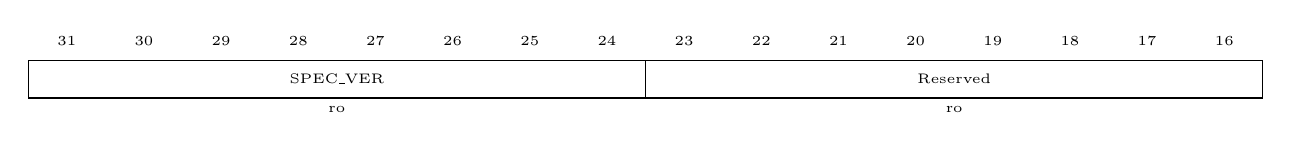
\begin{tikzpicture}[x=0.98cm,y=0.6cm]
\node[font=\tiny] at (0.5,1.2) {31};
\node[font=\tiny] at (1.5,1.2) {30};
\node[font=\tiny] at (2.5,1.2) {29};
\node[font=\tiny] at (3.5,1.2) {28};
\node[font=\tiny] at (4.5,1.2) {27};
\node[font=\tiny] at (5.5,1.2) {26};
\node[font=\tiny] at (6.5,1.2) {25};
\node[font=\tiny] at (7.5,1.2) {24};
\node[font=\tiny] at (8.5,1.2) {23};
\node[font=\tiny] at (9.5,1.2) {22};
\node[font=\tiny] at (10.5,1.2) {21};
\node[font=\tiny] at (11.5,1.2) {20};
\node[font=\tiny] at (12.5,1.2) {19};
\node[font=\tiny] at (13.5,1.2) {18};
\node[font=\tiny] at (14.5,1.2) {17};
\node[font=\tiny] at (15.5,1.2) {16};
\draw (0,0) rectangle (8,0.8);
\node[font=\tiny] at (4.0,0.4) {SPEC\_VER};
\node[font=\tiny] at (4.0,-0.25) {ro};
\draw (8,0) rectangle (16,0.8);
\node[font=\tiny] at (12.0,0.4) {Reserved};
\node[font=\tiny] at (12.0,-0.25) {ro};
\end{tikzpicture}
\end{center}
\begin{center}
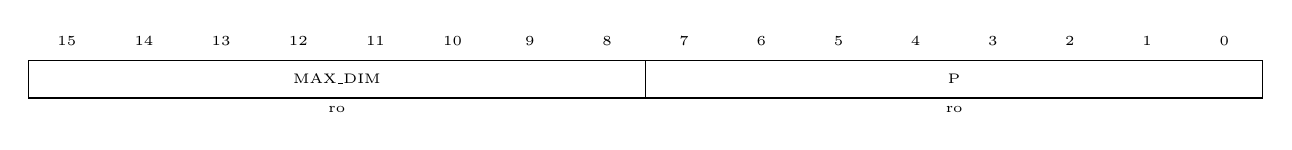
\begin{tikzpicture}[x=0.98cm,y=0.6cm]
\node[font=\tiny] at (0.5,1.2) {15};
\node[font=\tiny] at (1.5,1.2) {14};
\node[font=\tiny] at (2.5,1.2) {13};
\node[font=\tiny] at (3.5,1.2) {12};
\node[font=\tiny] at (4.5,1.2) {11};
\node[font=\tiny] at (5.5,1.2) {10};
\node[font=\tiny] at (6.5,1.2) {9};
\node[font=\tiny] at (7.5,1.2) {8};
\node[font=\tiny] at (8.5,1.2) {7};
\node[font=\tiny] at (9.5,1.2) {6};
\node[font=\tiny] at (10.5,1.2) {5};
\node[font=\tiny] at (11.5,1.2) {4};
\node[font=\tiny] at (12.5,1.2) {3};
\node[font=\tiny] at (13.5,1.2) {2};
\node[font=\tiny] at (14.5,1.2) {1};
\node[font=\tiny] at (15.5,1.2) {0};
\draw (0,0) rectangle (8,0.8);
\node[font=\tiny] at (4.0,0.4) {MAX\_DIM};
\node[font=\tiny] at (4.0,-0.25) {ro};
\draw (8,0) rectangle (16,0.8);
\node[font=\tiny] at (12.0,0.4) {P};
\node[font=\tiny] at (12.0,-0.25) {ro};
\end{tikzpicture}
\end{center}
\begin{spectable}{|L{0.09}|L{0.24}|L{0.08}|L{0.15}|L{0.44}|}{Cấu hình phần cứng}{reg:HW_CONFIG}{\textbf{Bit} & \textbf{Tên} & \textbf{Kiểu} & \textbf{Giá trị mặc định} & \textbf{Mô tả}}
31:24 & SPEC\_VER & RO & 8'h11 & Phiên bản giao diện phần cứng. 0x11: chỉ chuỗi descriptor và scratchpad ping-pong. \\\hline

23:16 & Reserved & RO & 8'h0 & Đọc 0; ghi bị bỏ qua. \\\hline

15:8 & MAX\_DIM & RO & 8'd32 & Kích thước ma trận tối đa của một descriptor. \\\hline

7:0 & P & RO & 8'd8 & Kích thước array; luôn bằng 8. \\\hline

\end{spectable}

\begin{notebox}[Quyết định baseline D-03]
Hai nguồn cho hai giá trị reset khác nhau: \sig{spec_1} dùng \{8'h11, 8'h00, 8'd32, P\} với
SPEC\_VER = 0x11 nghĩa là "chỉ chuỗi descriptor và ping-pong"; \sig{spec_2} dùng 0x1003\_2008 với
SPEC\_VER = 0x10 và thêm hai bit tính năng \sig{HAS_CHAIN} = bit 16, \sig{HAS_PINGPONG} = bit 17.
Baseline chọn \sig{spec_1} với P chốt bằng 8, tức giá trị reset \textbf{0x1100\_2008}.
Lý do: khi chuỗi descriptor và ping-pong là chế độ duy nhất (D-01), hai bit \sig{HAS_*} là hằng số 1
và không mang thông tin, trong khi SPEC\_VER = 0x11 đã mã hóa đúng khả năng đó bằng một trường duy
nhất. Giữ cả hai cách mô tả cùng một việc tạo ra hai nguồn sự thật cho firmware. Tác động:
bit [23:16] là Reserved đọc 0; firmware nhận biết khả năng của phần cứng qua SPEC\_VER.
\end{notebox}

\subsection{Tổng số chu kỳ BUSY của tác vụ (PERF\_TOTAL)}
Địa chỉ offset: 0x2C\par
Giá trị reset: 0x0000\_0000\par
\begin{center}
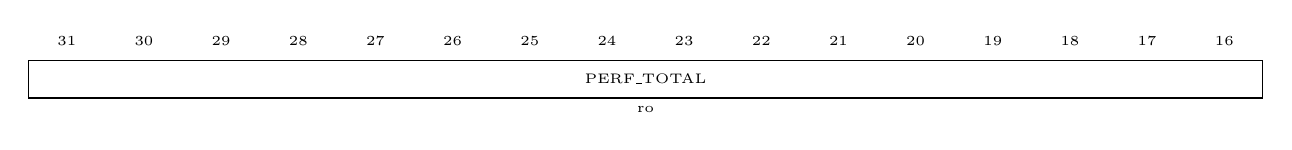
\begin{tikzpicture}[x=0.98cm,y=0.6cm]
\node[font=\tiny] at (0.5,1.2) {31};
\node[font=\tiny] at (1.5,1.2) {30};
\node[font=\tiny] at (2.5,1.2) {29};
\node[font=\tiny] at (3.5,1.2) {28};
\node[font=\tiny] at (4.5,1.2) {27};
\node[font=\tiny] at (5.5,1.2) {26};
\node[font=\tiny] at (6.5,1.2) {25};
\node[font=\tiny] at (7.5,1.2) {24};
\node[font=\tiny] at (8.5,1.2) {23};
\node[font=\tiny] at (9.5,1.2) {22};
\node[font=\tiny] at (10.5,1.2) {21};
\node[font=\tiny] at (11.5,1.2) {20};
\node[font=\tiny] at (12.5,1.2) {19};
\node[font=\tiny] at (13.5,1.2) {18};
\node[font=\tiny] at (14.5,1.2) {17};
\node[font=\tiny] at (15.5,1.2) {16};
\draw (0,0) rectangle (16,0.8);
\node[font=\tiny] at (8.0,0.4) {PERF\_TOTAL};
\node[font=\tiny] at (8.0,-0.25) {ro};
\end{tikzpicture}
\end{center}
\begin{center}
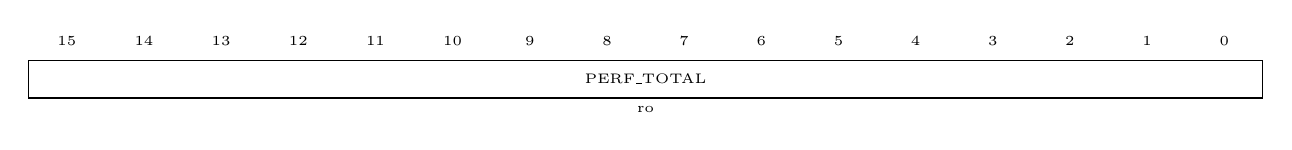
\begin{tikzpicture}[x=0.98cm,y=0.6cm]
\node[font=\tiny] at (0.5,1.2) {15};
\node[font=\tiny] at (1.5,1.2) {14};
\node[font=\tiny] at (2.5,1.2) {13};
\node[font=\tiny] at (3.5,1.2) {12};
\node[font=\tiny] at (4.5,1.2) {11};
\node[font=\tiny] at (5.5,1.2) {10};
\node[font=\tiny] at (6.5,1.2) {9};
\node[font=\tiny] at (7.5,1.2) {8};
\node[font=\tiny] at (8.5,1.2) {7};
\node[font=\tiny] at (9.5,1.2) {6};
\node[font=\tiny] at (10.5,1.2) {5};
\node[font=\tiny] at (11.5,1.2) {4};
\node[font=\tiny] at (12.5,1.2) {3};
\node[font=\tiny] at (13.5,1.2) {2};
\node[font=\tiny] at (14.5,1.2) {1};
\node[font=\tiny] at (15.5,1.2) {0};
\draw (0,0) rectangle (16,0.8);
\node[font=\tiny] at (8.0,0.4) {PERF\_TOTAL};
\node[font=\tiny] at (8.0,-0.25) {ro};
\end{tikzpicture}
\end{center}
\begin{spectable}{|L{0.09}|L{0.24}|L{0.08}|L{0.15}|L{0.44}|}{Tổng số chu kỳ BUSY của tác vụ}{reg:PERF_TOTAL}{\textbf{Bit} & \textbf{Tên} & \textbf{Kiểu} & \textbf{Giá trị mặc định} & \textbf{Mô tả}}
31:0 & PERF\_TOTAL & RO & 32'h0 & Tổng số chu kỳ BUSY của tác vụ. Về 0 ở chu kỳ START được chấp nhận; đếm trong lúc BUSY = 1; bão hòa tại 0xFFFF\_FFFF; giữ giá trị sau khi tác vụ kết thúc. \\\hline

\end{spectable}

\subsection{Số chu kỳ LOAD của tác vụ, không tính FETCH (PERF\_LOAD)}
Địa chỉ offset: 0x30\par
Giá trị reset: 0x0000\_0000\par
\begin{center}
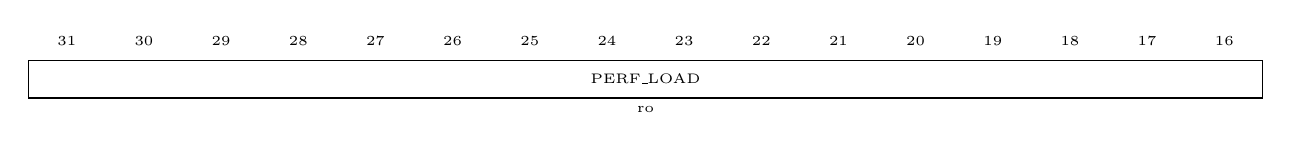
\begin{tikzpicture}[x=0.98cm,y=0.6cm]
\node[font=\tiny] at (0.5,1.2) {31};
\node[font=\tiny] at (1.5,1.2) {30};
\node[font=\tiny] at (2.5,1.2) {29};
\node[font=\tiny] at (3.5,1.2) {28};
\node[font=\tiny] at (4.5,1.2) {27};
\node[font=\tiny] at (5.5,1.2) {26};
\node[font=\tiny] at (6.5,1.2) {25};
\node[font=\tiny] at (7.5,1.2) {24};
\node[font=\tiny] at (8.5,1.2) {23};
\node[font=\tiny] at (9.5,1.2) {22};
\node[font=\tiny] at (10.5,1.2) {21};
\node[font=\tiny] at (11.5,1.2) {20};
\node[font=\tiny] at (12.5,1.2) {19};
\node[font=\tiny] at (13.5,1.2) {18};
\node[font=\tiny] at (14.5,1.2) {17};
\node[font=\tiny] at (15.5,1.2) {16};
\draw (0,0) rectangle (16,0.8);
\node[font=\tiny] at (8.0,0.4) {PERF\_LOAD};
\node[font=\tiny] at (8.0,-0.25) {ro};
\end{tikzpicture}
\end{center}
\begin{center}
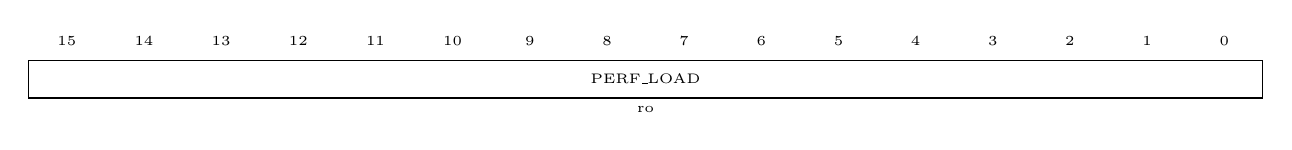
\begin{tikzpicture}[x=0.98cm,y=0.6cm]
\node[font=\tiny] at (0.5,1.2) {15};
\node[font=\tiny] at (1.5,1.2) {14};
\node[font=\tiny] at (2.5,1.2) {13};
\node[font=\tiny] at (3.5,1.2) {12};
\node[font=\tiny] at (4.5,1.2) {11};
\node[font=\tiny] at (5.5,1.2) {10};
\node[font=\tiny] at (6.5,1.2) {9};
\node[font=\tiny] at (7.5,1.2) {8};
\node[font=\tiny] at (8.5,1.2) {7};
\node[font=\tiny] at (9.5,1.2) {6};
\node[font=\tiny] at (10.5,1.2) {5};
\node[font=\tiny] at (11.5,1.2) {4};
\node[font=\tiny] at (12.5,1.2) {3};
\node[font=\tiny] at (13.5,1.2) {2};
\node[font=\tiny] at (14.5,1.2) {1};
\node[font=\tiny] at (15.5,1.2) {0};
\draw (0,0) rectangle (16,0.8);
\node[font=\tiny] at (8.0,0.4) {PERF\_LOAD};
\node[font=\tiny] at (8.0,-0.25) {ro};
\end{tikzpicture}
\end{center}
\begin{spectable}{|L{0.09}|L{0.24}|L{0.08}|L{0.15}|L{0.44}|}{Số chu kỳ LOAD của tác vụ, không tính FETCH}{reg:PERF_LOAD}{\textbf{Bit} & \textbf{Tên} & \textbf{Kiểu} & \textbf{Giá trị mặc định} & \textbf{Mô tả}}
31:0 & PERF\_LOAD & RO & 32'h0 & Số chu kỳ LOAD của tác vụ, không tính FETCH. Về 0 ở chu kỳ START được chấp nhận; tăng ở mỗi chu kỳ BUSY = 1 có pha LOAD đang chạy (\sig{i_perf_load} = 1); bão hòa tại 0xFFFF\_FFFF; giữ giá trị sau khi tác vụ kết thúc. \\\hline

\end{spectable}

\subsection{Số chu kỳ COMPUTE của tác vụ (PERF\_COMPUTE)}
Địa chỉ offset: 0x34\par
Giá trị reset: 0x0000\_0000\par
\begin{center}
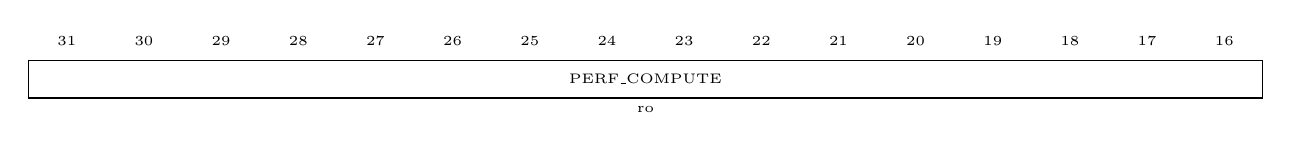
\begin{tikzpicture}[x=0.98cm,y=0.6cm]
\node[font=\tiny] at (0.5,1.2) {31};
\node[font=\tiny] at (1.5,1.2) {30};
\node[font=\tiny] at (2.5,1.2) {29};
\node[font=\tiny] at (3.5,1.2) {28};
\node[font=\tiny] at (4.5,1.2) {27};
\node[font=\tiny] at (5.5,1.2) {26};
\node[font=\tiny] at (6.5,1.2) {25};
\node[font=\tiny] at (7.5,1.2) {24};
\node[font=\tiny] at (8.5,1.2) {23};
\node[font=\tiny] at (9.5,1.2) {22};
\node[font=\tiny] at (10.5,1.2) {21};
\node[font=\tiny] at (11.5,1.2) {20};
\node[font=\tiny] at (12.5,1.2) {19};
\node[font=\tiny] at (13.5,1.2) {18};
\node[font=\tiny] at (14.5,1.2) {17};
\node[font=\tiny] at (15.5,1.2) {16};
\draw (0,0) rectangle (16,0.8);
\node[font=\tiny] at (8.0,0.4) {PERF\_COMPUTE};
\node[font=\tiny] at (8.0,-0.25) {ro};
\end{tikzpicture}
\end{center}
\begin{center}
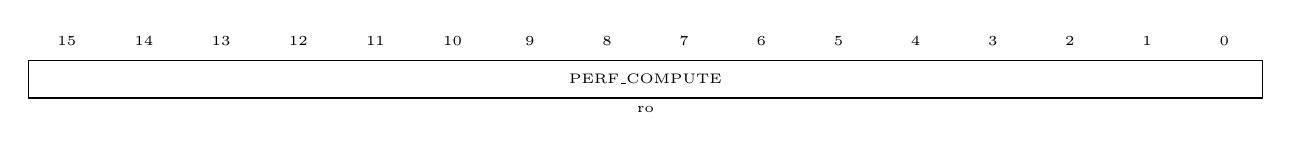
\begin{tikzpicture}[x=0.98cm,y=0.6cm]
\node[font=\tiny] at (0.5,1.2) {15};
\node[font=\tiny] at (1.5,1.2) {14};
\node[font=\tiny] at (2.5,1.2) {13};
\node[font=\tiny] at (3.5,1.2) {12};
\node[font=\tiny] at (4.5,1.2) {11};
\node[font=\tiny] at (5.5,1.2) {10};
\node[font=\tiny] at (6.5,1.2) {9};
\node[font=\tiny] at (7.5,1.2) {8};
\node[font=\tiny] at (8.5,1.2) {7};
\node[font=\tiny] at (9.5,1.2) {6};
\node[font=\tiny] at (10.5,1.2) {5};
\node[font=\tiny] at (11.5,1.2) {4};
\node[font=\tiny] at (12.5,1.2) {3};
\node[font=\tiny] at (13.5,1.2) {2};
\node[font=\tiny] at (14.5,1.2) {1};
\node[font=\tiny] at (15.5,1.2) {0};
\draw (0,0) rectangle (16,0.8);
\node[font=\tiny] at (8.0,0.4) {PERF\_COMPUTE};
\node[font=\tiny] at (8.0,-0.25) {ro};
\end{tikzpicture}
\end{center}
\begin{spectable}{|L{0.09}|L{0.24}|L{0.08}|L{0.15}|L{0.44}|}{Số chu kỳ COMPUTE của tác vụ}{reg:PERF_COMPUTE}{\textbf{Bit} & \textbf{Tên} & \textbf{Kiểu} & \textbf{Giá trị mặc định} & \textbf{Mô tả}}
31:0 & PERF\_COMPUTE & RO & 32'h0 & Số chu kỳ COMPUTE của tác vụ. Về 0 ở chu kỳ START được chấp nhận; tăng ở mỗi chu kỳ BUSY = 1 có pha COMPUTE đang chạy (\sig{i_perf_comp} = 1); bão hòa tại 0xFFFF\_FFFF; giữ giá trị sau khi tác vụ kết thúc. \\\hline

\end{spectable}

\subsection{Số chu kỳ STORE\_C của tác vụ (PERF\_STORE)}
Địa chỉ offset: 0x38\par
Giá trị reset: 0x0000\_0000\par
\begin{center}
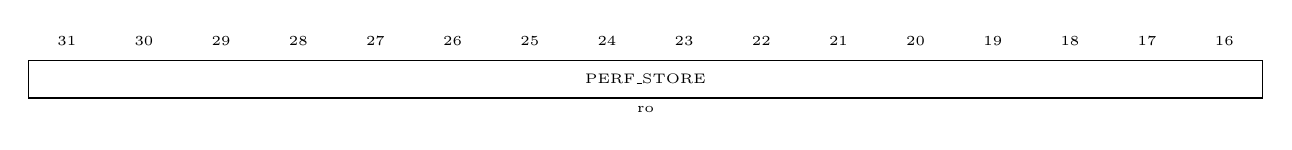
\begin{tikzpicture}[x=0.98cm,y=0.6cm]
\node[font=\tiny] at (0.5,1.2) {31};
\node[font=\tiny] at (1.5,1.2) {30};
\node[font=\tiny] at (2.5,1.2) {29};
\node[font=\tiny] at (3.5,1.2) {28};
\node[font=\tiny] at (4.5,1.2) {27};
\node[font=\tiny] at (5.5,1.2) {26};
\node[font=\tiny] at (6.5,1.2) {25};
\node[font=\tiny] at (7.5,1.2) {24};
\node[font=\tiny] at (8.5,1.2) {23};
\node[font=\tiny] at (9.5,1.2) {22};
\node[font=\tiny] at (10.5,1.2) {21};
\node[font=\tiny] at (11.5,1.2) {20};
\node[font=\tiny] at (12.5,1.2) {19};
\node[font=\tiny] at (13.5,1.2) {18};
\node[font=\tiny] at (14.5,1.2) {17};
\node[font=\tiny] at (15.5,1.2) {16};
\draw (0,0) rectangle (16,0.8);
\node[font=\tiny] at (8.0,0.4) {PERF\_STORE};
\node[font=\tiny] at (8.0,-0.25) {ro};
\end{tikzpicture}
\end{center}
\begin{center}
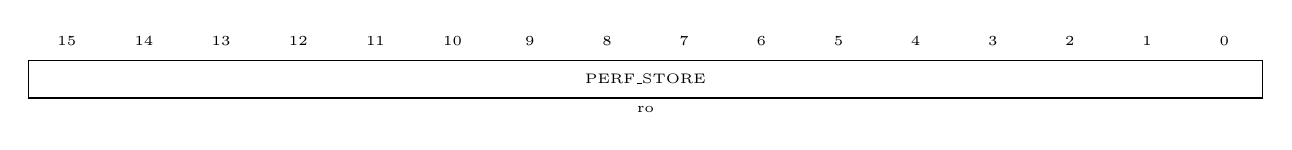
\begin{tikzpicture}[x=0.98cm,y=0.6cm]
\node[font=\tiny] at (0.5,1.2) {15};
\node[font=\tiny] at (1.5,1.2) {14};
\node[font=\tiny] at (2.5,1.2) {13};
\node[font=\tiny] at (3.5,1.2) {12};
\node[font=\tiny] at (4.5,1.2) {11};
\node[font=\tiny] at (5.5,1.2) {10};
\node[font=\tiny] at (6.5,1.2) {9};
\node[font=\tiny] at (7.5,1.2) {8};
\node[font=\tiny] at (8.5,1.2) {7};
\node[font=\tiny] at (9.5,1.2) {6};
\node[font=\tiny] at (10.5,1.2) {5};
\node[font=\tiny] at (11.5,1.2) {4};
\node[font=\tiny] at (12.5,1.2) {3};
\node[font=\tiny] at (13.5,1.2) {2};
\node[font=\tiny] at (14.5,1.2) {1};
\node[font=\tiny] at (15.5,1.2) {0};
\draw (0,0) rectangle (16,0.8);
\node[font=\tiny] at (8.0,0.4) {PERF\_STORE};
\node[font=\tiny] at (8.0,-0.25) {ro};
\end{tikzpicture}
\end{center}
\begin{spectable}{|L{0.09}|L{0.24}|L{0.08}|L{0.15}|L{0.44}|}{Số chu kỳ STORE\_C của tác vụ}{reg:PERF_STORE}{\textbf{Bit} & \textbf{Tên} & \textbf{Kiểu} & \textbf{Giá trị mặc định} & \textbf{Mô tả}}
31:0 & PERF\_STORE & RO & 32'h0 & Số chu kỳ STORE\_C của tác vụ. Về 0 ở chu kỳ START được chấp nhận; tăng ở mỗi chu kỳ BUSY = 1 có pha STORE\_C đang chạy (\sig{i_perf_store} = 1); bão hòa tại 0xFFFF\_FFFF; giữ giá trị sau khi tác vụ kết thúc. \\\hline

\end{spectable}

\subsection{Con trỏ descriptor đầu (DESC\_PTR)}
Địa chỉ offset: 0x40\par
Giá trị reset: 0x0000\_0000\par
\begin{center}
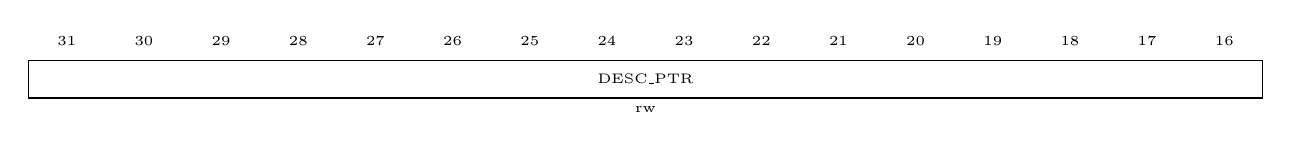
\begin{tikzpicture}[x=0.98cm,y=0.6cm]
\node[font=\tiny] at (0.5,1.2) {31};
\node[font=\tiny] at (1.5,1.2) {30};
\node[font=\tiny] at (2.5,1.2) {29};
\node[font=\tiny] at (3.5,1.2) {28};
\node[font=\tiny] at (4.5,1.2) {27};
\node[font=\tiny] at (5.5,1.2) {26};
\node[font=\tiny] at (6.5,1.2) {25};
\node[font=\tiny] at (7.5,1.2) {24};
\node[font=\tiny] at (8.5,1.2) {23};
\node[font=\tiny] at (9.5,1.2) {22};
\node[font=\tiny] at (10.5,1.2) {21};
\node[font=\tiny] at (11.5,1.2) {20};
\node[font=\tiny] at (12.5,1.2) {19};
\node[font=\tiny] at (13.5,1.2) {18};
\node[font=\tiny] at (14.5,1.2) {17};
\node[font=\tiny] at (15.5,1.2) {16};
\draw (0,0) rectangle (16,0.8);
\node[font=\tiny] at (8.0,0.4) {DESC\_PTR};
\node[font=\tiny] at (8.0,-0.25) {rw};
\end{tikzpicture}
\end{center}
\begin{center}
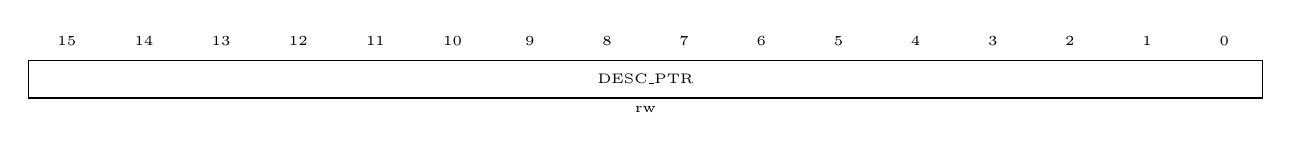
\begin{tikzpicture}[x=0.98cm,y=0.6cm]
\node[font=\tiny] at (0.5,1.2) {15};
\node[font=\tiny] at (1.5,1.2) {14};
\node[font=\tiny] at (2.5,1.2) {13};
\node[font=\tiny] at (3.5,1.2) {12};
\node[font=\tiny] at (4.5,1.2) {11};
\node[font=\tiny] at (5.5,1.2) {10};
\node[font=\tiny] at (6.5,1.2) {9};
\node[font=\tiny] at (7.5,1.2) {8};
\node[font=\tiny] at (8.5,1.2) {7};
\node[font=\tiny] at (9.5,1.2) {6};
\node[font=\tiny] at (10.5,1.2) {5};
\node[font=\tiny] at (11.5,1.2) {4};
\node[font=\tiny] at (12.5,1.2) {3};
\node[font=\tiny] at (13.5,1.2) {2};
\node[font=\tiny] at (14.5,1.2) {1};
\node[font=\tiny] at (15.5,1.2) {0};
\draw (0,0) rectangle (16,0.8);
\node[font=\tiny] at (8.0,0.4) {DESC\_PTR};
\node[font=\tiny] at (8.0,-0.25) {rw};
\end{tikzpicture}
\end{center}
\begin{spectable}{|L{0.09}|L{0.24}|L{0.08}|L{0.15}|L{0.44}|}{Con trỏ descriptor đầu}{reg:DESC_PTR}{\textbf{Bit} & \textbf{Tên} & \textbf{Kiểu} & \textbf{Giá trị mặc định} & \textbf{Mô tả}}
31:0 & DESC\_PTR & RW & 32'h0 & Địa chỉ byte của descriptor đầu chuỗi; phải căn 64 byte. Lưu đủ 32 bit. Ghi được bất kỳ lúc nào, kể cả khi BUSY = 1; đọc lại trả về giá trị CPU đã ghi, không phải bản chụp. Giá trị mới áp dụng từ lần START được chấp nhận tiếp theo. Soft reset giữ nguyên thanh ghi này. \\\hline

\end{spectable}

\subsection{Địa chỉ descriptor lỗi (ERR\_DESC\_ADDR)}
Địa chỉ offset: 0x44\par
Giá trị reset: 0x0000\_0000\par
\begin{center}
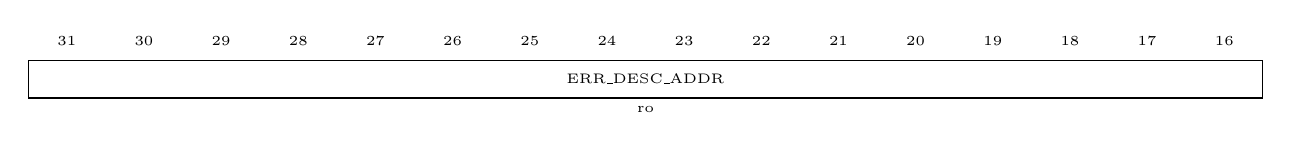
\begin{tikzpicture}[x=0.98cm,y=0.6cm]
\node[font=\tiny] at (0.5,1.2) {31};
\node[font=\tiny] at (1.5,1.2) {30};
\node[font=\tiny] at (2.5,1.2) {29};
\node[font=\tiny] at (3.5,1.2) {28};
\node[font=\tiny] at (4.5,1.2) {27};
\node[font=\tiny] at (5.5,1.2) {26};
\node[font=\tiny] at (6.5,1.2) {25};
\node[font=\tiny] at (7.5,1.2) {24};
\node[font=\tiny] at (8.5,1.2) {23};
\node[font=\tiny] at (9.5,1.2) {22};
\node[font=\tiny] at (10.5,1.2) {21};
\node[font=\tiny] at (11.5,1.2) {20};
\node[font=\tiny] at (12.5,1.2) {19};
\node[font=\tiny] at (13.5,1.2) {18};
\node[font=\tiny] at (14.5,1.2) {17};
\node[font=\tiny] at (15.5,1.2) {16};
\draw (0,0) rectangle (16,0.8);
\node[font=\tiny] at (8.0,0.4) {ERR\_DESC\_ADDR};
\node[font=\tiny] at (8.0,-0.25) {ro};
\end{tikzpicture}
\end{center}
\begin{center}
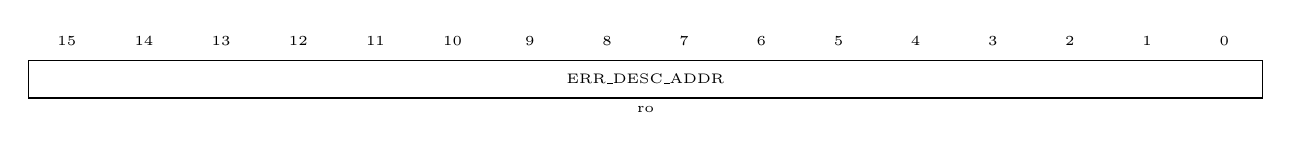
\begin{tikzpicture}[x=0.98cm,y=0.6cm]
\node[font=\tiny] at (0.5,1.2) {15};
\node[font=\tiny] at (1.5,1.2) {14};
\node[font=\tiny] at (2.5,1.2) {13};
\node[font=\tiny] at (3.5,1.2) {12};
\node[font=\tiny] at (4.5,1.2) {11};
\node[font=\tiny] at (5.5,1.2) {10};
\node[font=\tiny] at (6.5,1.2) {9};
\node[font=\tiny] at (7.5,1.2) {8};
\node[font=\tiny] at (8.5,1.2) {7};
\node[font=\tiny] at (9.5,1.2) {6};
\node[font=\tiny] at (10.5,1.2) {5};
\node[font=\tiny] at (11.5,1.2) {4};
\node[font=\tiny] at (12.5,1.2) {3};
\node[font=\tiny] at (13.5,1.2) {2};
\node[font=\tiny] at (14.5,1.2) {1};
\node[font=\tiny] at (15.5,1.2) {0};
\draw (0,0) rectangle (16,0.8);
\node[font=\tiny] at (8.0,0.4) {ERR\_DESC\_ADDR};
\node[font=\tiny] at (8.0,-0.25) {ro};
\end{tikzpicture}
\end{center}
\begin{spectable}{|L{0.09}|L{0.24}|L{0.08}|L{0.15}|L{0.44}|}{Địa chỉ descriptor lỗi}{reg:ERR_DESC_ADDR}{\textbf{Bit} & \textbf{Tên} & \textbf{Kiểu} & \textbf{Giá trị mặc định} & \textbf{Mô tả}}
31:0 & ERR\_DESC\_ADDR & RO & 32'h0 & Địa chỉ của descriptor có lỗi sớm nhất theo thứ tự chuỗi. Chỉ có nghĩa khi ERROR = 1. Xóa khi nhận tác vụ mới, khi soft reset hoặc khi reset. \\\hline

\end{spectable}

\subsection{Số descriptor hoàn tất (DESC\_DONE\_CNT)}
Địa chỉ offset: 0x48\par
Giá trị reset: 0x0000\_0000\par
\begin{center}
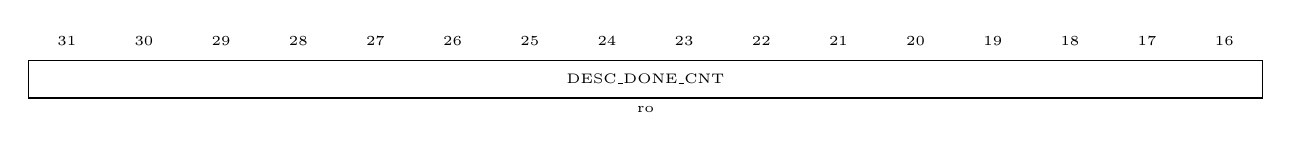
\begin{tikzpicture}[x=0.98cm,y=0.6cm]
\node[font=\tiny] at (0.5,1.2) {31};
\node[font=\tiny] at (1.5,1.2) {30};
\node[font=\tiny] at (2.5,1.2) {29};
\node[font=\tiny] at (3.5,1.2) {28};
\node[font=\tiny] at (4.5,1.2) {27};
\node[font=\tiny] at (5.5,1.2) {26};
\node[font=\tiny] at (6.5,1.2) {25};
\node[font=\tiny] at (7.5,1.2) {24};
\node[font=\tiny] at (8.5,1.2) {23};
\node[font=\tiny] at (9.5,1.2) {22};
\node[font=\tiny] at (10.5,1.2) {21};
\node[font=\tiny] at (11.5,1.2) {20};
\node[font=\tiny] at (12.5,1.2) {19};
\node[font=\tiny] at (13.5,1.2) {18};
\node[font=\tiny] at (14.5,1.2) {17};
\node[font=\tiny] at (15.5,1.2) {16};
\draw (0,0) rectangle (16,0.8);
\node[font=\tiny] at (8.0,0.4) {DESC\_DONE\_CNT};
\node[font=\tiny] at (8.0,-0.25) {ro};
\end{tikzpicture}
\end{center}
\begin{center}
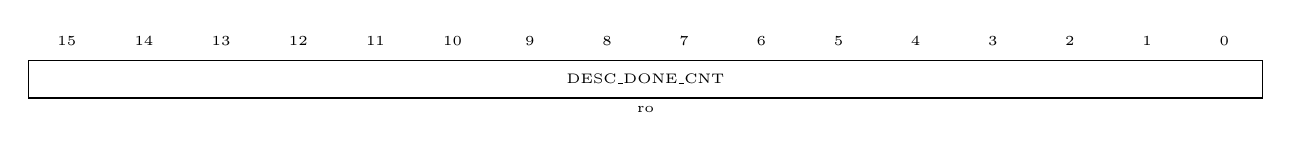
\begin{tikzpicture}[x=0.98cm,y=0.6cm]
\node[font=\tiny] at (0.5,1.2) {15};
\node[font=\tiny] at (1.5,1.2) {14};
\node[font=\tiny] at (2.5,1.2) {13};
\node[font=\tiny] at (3.5,1.2) {12};
\node[font=\tiny] at (4.5,1.2) {11};
\node[font=\tiny] at (5.5,1.2) {10};
\node[font=\tiny] at (6.5,1.2) {9};
\node[font=\tiny] at (7.5,1.2) {8};
\node[font=\tiny] at (8.5,1.2) {7};
\node[font=\tiny] at (9.5,1.2) {6};
\node[font=\tiny] at (10.5,1.2) {5};
\node[font=\tiny] at (11.5,1.2) {4};
\node[font=\tiny] at (12.5,1.2) {3};
\node[font=\tiny] at (13.5,1.2) {2};
\node[font=\tiny] at (14.5,1.2) {1};
\node[font=\tiny] at (15.5,1.2) {0};
\draw (0,0) rectangle (16,0.8);
\node[font=\tiny] at (8.0,0.4) {DESC\_DONE\_CNT};
\node[font=\tiny] at (8.0,-0.25) {ro};
\end{tikzpicture}
\end{center}
\begin{spectable}{|L{0.09}|L{0.24}|L{0.08}|L{0.15}|L{0.44}|}{Số descriptor hoàn tất}{reg:DESC_DONE_CNT}{\textbf{Bit} & \textbf{Tên} & \textbf{Kiểu} & \textbf{Giá trị mặc định} & \textbf{Mô tả}}
31:0 & DESC\_DONE\_CNT & RO & 32'h0 & Tăng 1 mỗi khi STORE\_C của một descriptor nhận phản hồi B cuối là OKAY; các descriptor hoàn tất đúng theo thứ tự chuỗi. Khi ERROR = 1, bằng số thứ tự của descriptor lỗi sớm nhất. Xóa khi nhận tác vụ mới, khi soft reset hoặc khi reset. \\\hline

\end{spectable}

\subsection{Mã lỗi}\label{sec:2.2}
\begin{spectable}{|L{0.12}|L{0.28}|L{0.6}|}{Mã lỗi \sigc{ERR_CODE} (STATUS[7:4])}{tab:2-2}{\textbf{Giá trị} & \textbf{Ý nghĩa} & \textbf{Khi nào xuất hiện}}
0 & Không lỗi & ERROR = 0 \\\hline

1 & Cấu hình sai & Descriptor sai điều kiện hợp lệ ở mục~\ref{sec:5.2}, hoặc \sig{DESC_PTR} không căn 64 byte \\\hline

2 & Lỗi AXI khi đọc & LOAD\_A, LOAD\_B hoặc LOAD\_BIAS gặp \sig{m_axi_rresp} ≠ OKAY hoặc \sig{m_axi_rlast} sai vị trí \\\hline

3 & Lỗi AXI khi ghi & STORE\_C gặp \sig{m_axi_bresp} ≠ OKAY \\\hline

4 & Lỗi AXI khi đọc descriptor & FETCH gặp \sig{m_axi_rresp} ≠ OKAY hoặc \sig{m_axi_rlast} sai vị trí \\\hline

5 … 15 & Dự trữ & Không bao giờ xuất hiện \\\hline

\end{spectable}

\begin{notebox}[Quyết định baseline D-02]
\sig{spec_2} định nghĩa thêm mã 5 "tính năng không có", đồng thời tự ghi rằng mã này không bao giờ
phát sinh vì chế độ chuỗi luôn bật. Baseline theo \sig{spec_1}: miền mã lỗi là 0 … 4, còn
5 … 15 dự trữ. Lý do: đây là hệ quả trực tiếp của D-01 — khi chỉ có một chế độ thì không tồn tại
tình huống "tính năng không có", nên một mã lỗi không thể phát sinh chỉ làm phức tạp bảng mã và
phần mềm xử lý lỗi.
\end{notebox}

\subsection{Yêu cầu thanh ghi}\label{sec:2.3}

\paragraph{Thanh ghi}\label{par:2-3}
\begin{itemize}
\item Offset, tên, quyền truy cập và giá trị reset đúng theo register map ở trên
\item \sig{CTRL[2]} START: ghi 1 bắt đầu chuỗi descriptor tại \sig{DESC_PTR}. Bit tự xóa, đọc luôn ra 0. Ghi 0 không có tác dụng. Ghi khi bận bị bỏ qua, không báo lỗi
\item \sig{CTRL[1]} SOFT\_RESET: ghi 1 là yêu cầu soft reset (mục~\ref{sec:4.5}); tự xóa. Một lần ghi CTRL có SOFT\_RESET = 1 thì chỉ SOFT\_RESET có hiệu lực, START trong cùng lệnh ghi bị bỏ qua
\item \sig{CTRL[0]} dự trữ: đọc 0, ghi bị bỏ qua. Các bit lệnh của CTRL chỉ có hiệu lực khi \sig{s_axi_wstrb[0]} = 1
\item \sig{ERR_CODE} = 0 khi ERROR = 0. \sig{STATUS[3]} luôn đọc ra 0
\item \sig{DESC_PTR} ghi được bất kỳ lúc nào, kể cả khi BUSY = 1. Đọc lại trả giá trị CPU đã ghi, không phải bản chụp. Giá trị mới áp dụng từ lần START được chấp nhận tiếp theo
\item Thanh ghi RW lưu đủ 32 bit, kể cả bit dự trữ. Bit dự trữ của CTRL và STATUS: ghi bị bỏ qua, đọc ra 0. Offset dự trữ, kể cả 0x08 … 0x24 và 0x3C: đọc ra 0, ghi bị bỏ qua. Ghi vào thanh ghi chỉ đọc bị bỏ qua. Mọi truy cập đều trả \sig{s_axi_bresp} / \sig{s_axi_rresp} = 2'b00 (OKAY)
\item \sig{rst_n} đưa mọi thanh ghi về giá trị reset. Soft reset giữ nguyên \sig{DESC_PTR} và các thanh ghi RW; xóa \sig{STATUS}, \sig{PERF_*}, \sig{ERR_DESC_ADDR} và \sig{DESC_DONE_CNT}
\item \sig{PERF_*} về 0 ở chu kỳ START được chấp nhận; \sig{PERF_TOTAL} đếm mọi chu kỳ BUSY = 1, \sig{PERF_LOAD}, \sig{PERF_COMPUTE}, \sig{PERF_STORE} chỉ đếm chu kỳ BUSY = 1 có pha tương ứng đang chạy; dừng khi tác vụ kết thúc, bão hòa ở 0xFFFF\_FFFF. Khi các pha chồng nhau, \sig{PERF_LOAD} + \sig{PERF_COMPUTE} + \sig{PERF_STORE} có thể lớn hơn \sig{PERF_TOTAL}; phần chênh là thời gian chạy chồng
\item \sig{DESC_PTR} được chụp ở chu kỳ START được chấp nhận và giữ ổn định tới hết tác vụ. Nếu bit [5:0] của bản chụp khác 0, tác vụ kết thúc với \sig{ERR_CODE} = 1 và \textbf{không} truy cập bus, \textbf{không} truy cập scratchpad
\end{itemize}

\subsection{Ngữ nghĩa tác vụ}\label{sec:2.4}

\paragraph{Tác vụ}\label{par:2-4}
\begin{itemize}
\item START chỉ được chấp nhận nếu BUSY = 0 tại chu kỳ Register File thực hiện lệnh ghi CTRL. START khi BUSY = 1 bị bỏ qua, không đổi trạng thái, không báo lỗi
\item Ngay chu kỳ chấp nhận: Register File chụp \sig{DESC_PTR}; xóa DONE, ERROR, \sig{ERR_CODE}, \sig{PERF_*}. BUSY = 1 từ chu kỳ kế tiếp. \sig{ERR_DESC_ADDR} và \sig{DESC_DONE_CNT} nằm trong Main FSM và được xóa ở cạnh clock cuối chu kỳ có \sig{o_start_pulse}, tức chậm hơn một chu kỳ; CPU không quan sát được độ lệch này vì mọi lần đọc sau phản hồi B của lệnh ghi CTRL đều tới muộn hơn
\item Register File phát \sig{o_start_pulse} và chụp \sig{DESC_PTR} trước khi trả phản hồi B cho lệnh ghi CTRL; mọi lần đọc STATUS sau khi lệnh ghi hoàn tất đều thấy tác vụ mới
\item DONE = 1 chỉ khi STORE\_C của descriptor có \sig{LAST} = 1 đã nhận phản hồi B cuối là OKAY và không có lỗi nào trong cả chuỗi
\item ERROR được đặt khi đã có lỗi và mọi engine đã yên. Gọi f là descriptor lỗi sớm nhất theo thứ tự chuỗi: không pha mới nào của descriptor có chỉ số ≥ f được bắt đầu; mọi descriptor đứng trước f chạy xong, kể cả STORE\_C. \sig{ERR_DESC_ADDR} là địa chỉ của f; \sig{DESC_DONE_CNT} bằng f; vùng đích trong DRAM của descriptor ≥ f không xác định
\item BUSY về 0 ở đúng cạnh clock mà DONE hoặc ERROR được đặt. Sau khi chấp nhận và cho tới tác vụ kế tiếp hoặc soft reset, mọi lần đọc STATUS thấy đúng một trong ba bit BUSY, DONE, ERROR bằng 1
\item \sig{o_done_pulse} và \sig{o_err_pulse} không bao giờ xuất hiện trong cùng một chu kỳ
\item DONE và ERROR giữ giá trị (sticky); chỉ bị xóa khi tác vụ mới được chấp nhận, khi soft reset hoặc khi \sig{rst_n}
\item Sau DONE hoặc ERROR, firmware được phép ghi START ngay, không cần soft reset
\item Tín hiệu "xong" nội bộ (\sig{o_rd_done}, \sig{o_wr_done} của một lệnh DMA, \sig{o_pe_done} của array) không hiện ra cho CPU; chỉ \sig{STATUS}.DONE báo toàn bộ tác vụ xong
\end{itemize}

\subsection{Quy tắc cho firmware}\label{sec:2.5}

\paragraph{Firmware}\label{par:2-5}
\begin{itemize}
\item Trước lệnh ghi START, firmware ghi descriptor và dữ liệu vào DRAM, ghi \sig{DESC_PTR}, rồi thực hiện \sig{fence rw,rw}
\item Firmware chờ bằng polling cho tới khi DONE hoặc ERROR bằng 1, rồi thực hiện \sig{fence rw,rw} trước khi đọc kết quả
\item Đường DMA được giả định nhất quán cache với CPU. Nếu hệ thống tích hợp không bảo đảm điều đó, firmware phải flush dòng cache của descriptor, A, B và bias trước START, và hủy dòng cache của vùng đích sau DONE
\item Firmware không sửa descriptor và không ghi vào vùng DRAM của chuỗi đang chạy
\end{itemize}

\begin{Verbatim}[frame=leftline,framerule=2pt,rulecolor=\color{brand},xleftmargin=6pt,samepage=true]
#define GEMM_BASE  0x60000000u
#define REG(off)   (*(volatile uint32_t *)(GEMM_BASE + (off)))
#define ST_DONE    (1u << 0)
#define ST_ERROR   (1u << 2)

int gemm_run(uint32_t desc) {
    REG(0x40) = desc;                     /* DESC_PTR, căn 64 byte */
    asm volatile ("fence rw,rw");
    REG(0x00) = 4u;                       /* CTRL[2] = START */
    uint32_t s;
    do { s = REG(0x04); } while (!(s & (ST_DONE | ST_ERROR)));
    asm volatile ("fence rw,rw");
    return (s & ST_ERROR) ? (int)((s >> 4) & 0xFu) : 0;
}
\end{Verbatim}
